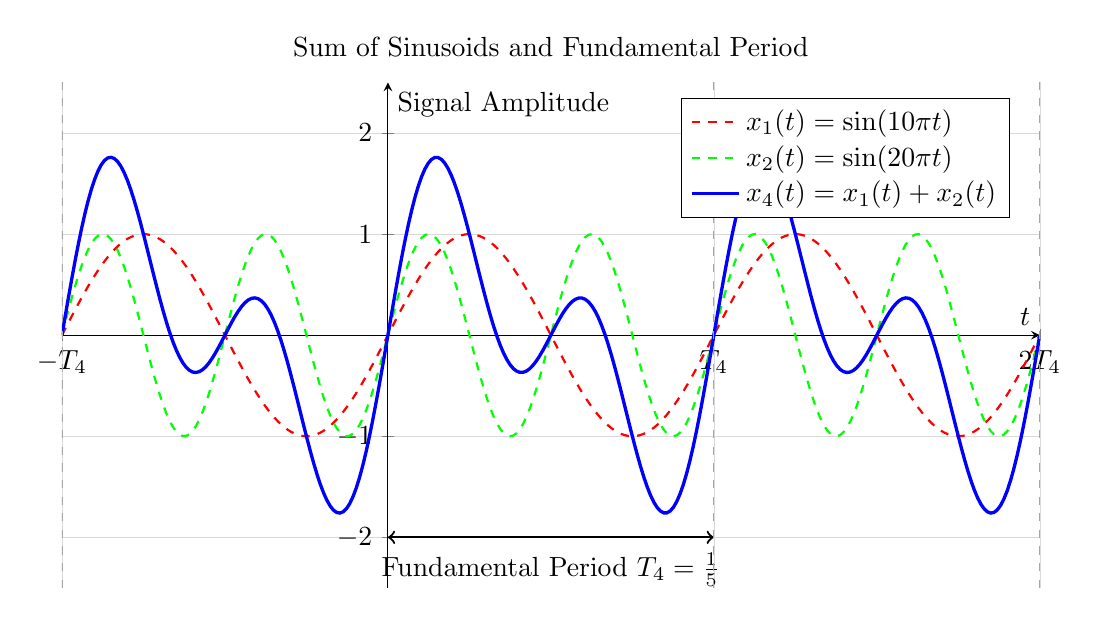
\begin{tikzpicture}
	\begin{axis}[
		% Set the overall style
		width=14cm,
		height=8cm,
		title={Sum of Sinusoids and Fundamental Period},
		% Axis labels
		axis lines=middle,
		xlabel={$t$},
		ylabel={Signal Amplitude},
		% Set axis limits to show one negative and two positive cycles
		xmin=-0.2, xmax=0.4,
		ymin=-2.5, ymax=2.5,
		% Use symbolic ticks including the negative period
		xtick={-0.2, 0.2, 0.4},
		xticklabels={$-T_4$, $T_4$, $2T_4$},
		ytick={-2, -1, 1, 2},
		% Add a grid
		grid=major,
		grid style={line width=.1pt, draw=gray!30},
		% Plotting settings
		domain=-0.2:0.4,
		samples=300,
		no marks,
		% Legend settings
		legend pos=north east,
		legend cell align={left},
		]
		
		% Plot the two component sinusoids (dashed and less thick)
		\addplot[red, thick, dashed] {sin(deg(10*pi*x))};
		\addlegendentry{$x_1(t) = \sin(10\pi t)$};
		
		\addplot[green, thick, dashed] {sin(deg(20*pi*x))};
		\addlegendentry{$x_2(t) = \sin(20\pi t)$};
		
		% Plot the sum (solid and very thick to emphasize it)
		\addplot[blue, very thick] {sin(deg(10*pi*x)) + sin(deg(20*pi*x))};
		\addlegendentry{$x_4(t) = x_1(t) + x_2(t)$};
		
		% Add a double-arrow line below the axis to mark the fundamental period
		\draw[<->, thick] (axis cs:0, -2) -- (axis cs:0.2, -2) 
		node[midway, below=2pt] {Fundamental Period $T_4 = \frac{1}{5}$};
		
		% Add subtle vertical lines to guide the eye at each period
		\draw[dashed, gray!70] (axis cs:-0.2, -2.5) -- (axis cs:-0.2, 2.5);
		\draw[dashed, gray!70] (axis cs:0.2, -2.5) -- (axis cs:0.2, 2.5);
		\draw[dashed, gray!70] (axis cs:0.4, -2.5) -- (axis cs:0.4, 2.5);
		
	\end{axis}
\end{tikzpicture}